% PROSZĘ KOMPILOWAĆ TEN DOKUMENT ZA POMOCĄ SILNIKA XELATEX
% W PRZECIWNYM RAZIE NALEŻY USUNĄĆ PAKIET fontspec ORAZ USTAWIENIA FONTU
% Z PLIKU styles/prez_wmini_pl.sty (PIERWSZE TRZY LINIJKI)
% W PRZYPADKU BRAKU FONTU Adagio Slab NALEŻY ZGŁOSIĆ SIĘ DO BIP PW O JEGO UDOSTĘPNIENIE,
% ZAŁADOWAĆ INNY KRÓJ CZCIONKI LUB ZAKOMENTOWAĆ/USUNĄĆ USTAWIENIA FONTU

\documentclass[aspectratio=169]{beamer}

\usepackage{styles/prez_wmini_pl}
\usepackage{booktabs}
\setbeamertemplate{section in toc}[sections numbered]
\setbeamertemplate{subsection in toc}[subsections numbered]
\usepackage{times}
\usepackage{amsmath}
\usepackage{bm}

\usefonttheme[onlymath]{serif}

\definecolor{quotationcolour}{HTML}{F0F0F0}
\definecolor{quotationmarkcolour}{HTML}{1F3F81}

% Double-line for start and end of epigraph.
\newcommand{\epiline}{\hrule \vskip -.2em \hrule}
% Massively humongous opening quotation mark.
\newcommand{\hugequote}{%
  \fontsize{42}{48}\selectfont \color{quotationmarkcolour} \textbf{``}
  \vskip -.5em
}

% Beautify quotations.
\newcommand{\epigraph}[2]{%
  \bigskip
  \begin{center}
  \colorbox{quotationcolour}{%
    \parbox{.80\textwidth}{%
    \epiline \vskip 1em {\hugequote} \vskip -.5em
    \parindent 2.2em
    #1\vspace{-.25cm}\begin{flushright}\textsc{#2}\end{flushright}
    \epiline
    }
  }
  \end{center}
  \bigskip
}

\newcommand{\boldm}[1] {\mathversion{bold}#1\mathversion{normal}}

\graphicspath{ {./images/} }



% ------------------ Ustawienia użytkownika ------------------
% kolor tytułu prezentacji; zalecany white lub grafitowy.
% Poza tym można użyć zdefiniowanych w pakiecie kolorów:
% sloneczny, morelowy, mietowy, mokka, grafitowy, sliwkowy, szafirowy, wrzosowy
% lub wybrać sobie kolor z pakietu xcolor
\colorlet{title_color}{grafitowy}

\title{Opracowanie wirtualnego środowiska\\do symulacji dynamiki lotu\\ bezzałogowych statków powietrznych}
%\subtitle{Podtytuł consectetur adispiscing elit}
\author{Wojciech Gajda \and  Igor Faliszewski}
\date{28 listopada 2023} % można tam wpisać datę jaką się chce lub zakomentować dla daty dzisiejszej



% ------------------ Początek prezentacji ------------------

\begin{document}
\sloppy

% Slajd tytułowy
{
\maketitleframe 
}

\begin{frame}
\frametitle{Agenda}
  \tableofcontents[  
    sectionstyle=show, 
    %hideallsubsections
    ]
\end{frame}

\section{Wprowadzenie}
\subsection{Motywacje}
\begin{frame}%[allowframebreaks]
	\frametitle{Motywacja}
	\begin{columns}
		\begin{column}{0.33\textwidth}
	   	 	\begin{figure}
	   		 \centering
	      		 \uncover<2->{
\includegraphics[width=0.9\textwidth]{logos/warthunder.png}}
	    		\end{figure}
	    		\begin{figure}
	   		 \centering
	      		 \uncover<3->{
\includegraphics[width=0.9\textwidth]{logos/MFS.png}}
	    		\end{figure}
		\end{column}
		\begin{column}{0.33\textwidth}
	   	 	\begin{figure}
	   		 \centering
	      		 \uncover<4->{
\includegraphics[width=0.9\textwidth]{logos/ardupilot.jpg}}
	    		\end{figure}
	    		\begin{figure}
	   		 \centering
	      		 \uncover<5->{
\includegraphics[width=0.9\textwidth]{logos/betaflight.png}}
	    		\end{figure}
	    		\begin{figure}
	   		 \centering
	      		 \uncover<6->{
\includegraphics[width=0.9\textwidth]{logos/inav.png}}
	    		\end{figure}
		\end{column}
		\begin{column}{0.33\textwidth}
	    		\begin{figure}
	   		 \centering
	      		 \uncover<7->{
\includegraphics[width=0.5\textwidth]{logos/JSBSim.png}}
	    		\end{figure}
			\begin{figure}
	   		 \centering
	      		 \uncover<8->{
\includegraphics[width=0.5\textwidth]{logos/VBS.png}}
	    		\end{figure}
		\end{column}
	\end{columns}
\end{frame}

\begin{frame}%[allowframebreaks]
	\frametitle{Motywacja}
	\begin{columns}
		\begin{column}{0.33\textwidth}
	   	 	\begin{figure}
	   		 \centering
	      		 \uncover<2->{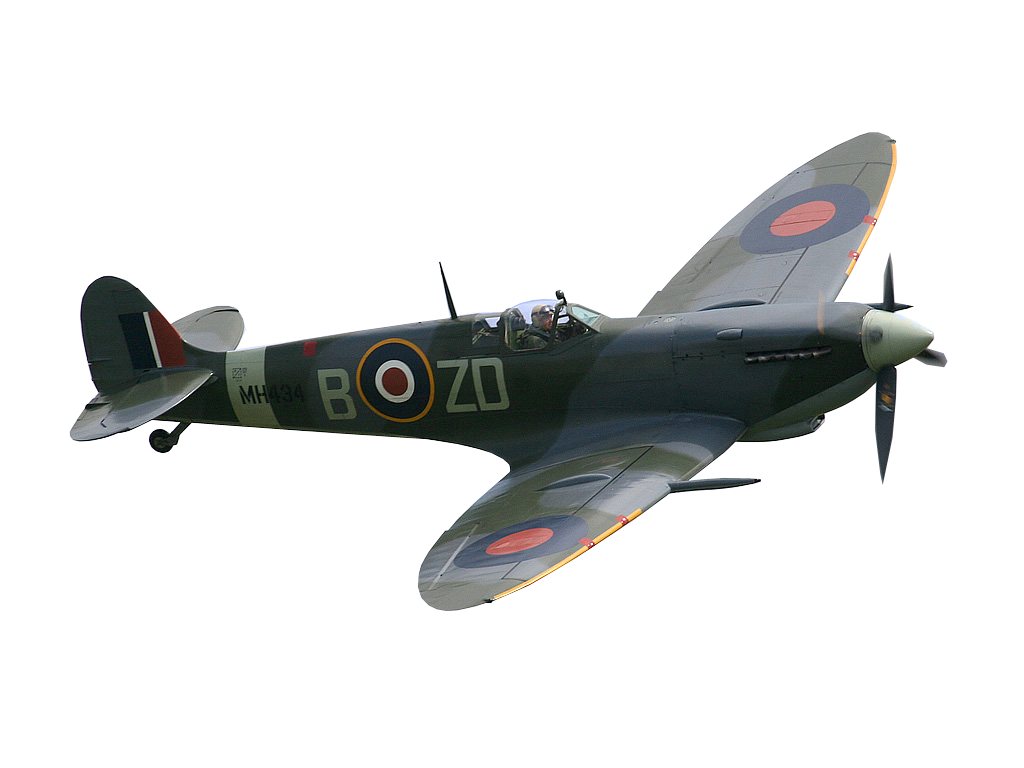
\includegraphics[width=0.9\textwidth]{spitfire.png}}
	    		\end{figure}
		\end{column}
		\begin{column}{0.33\textwidth}
	   	 	\begin{figure}
	   		 \centering
	      		 \uncover<3->{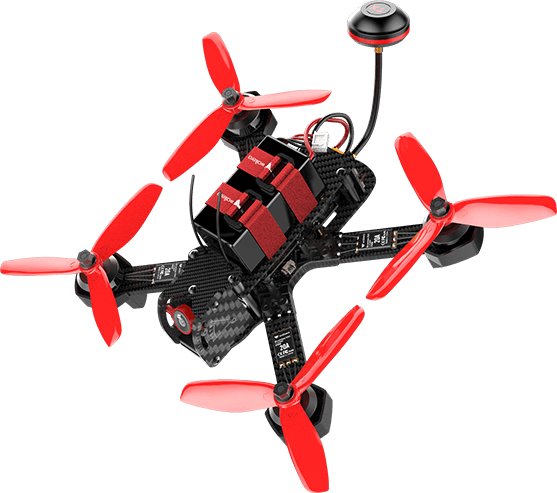
\includegraphics[width=0.9\textwidth]{quadcopter_fpv.png}}
	    		\end{figure}
		\end{column}
		\begin{column}{0.33\textwidth}
	    		\begin{figure}
	   		 \centering
	      		 \uncover<4->{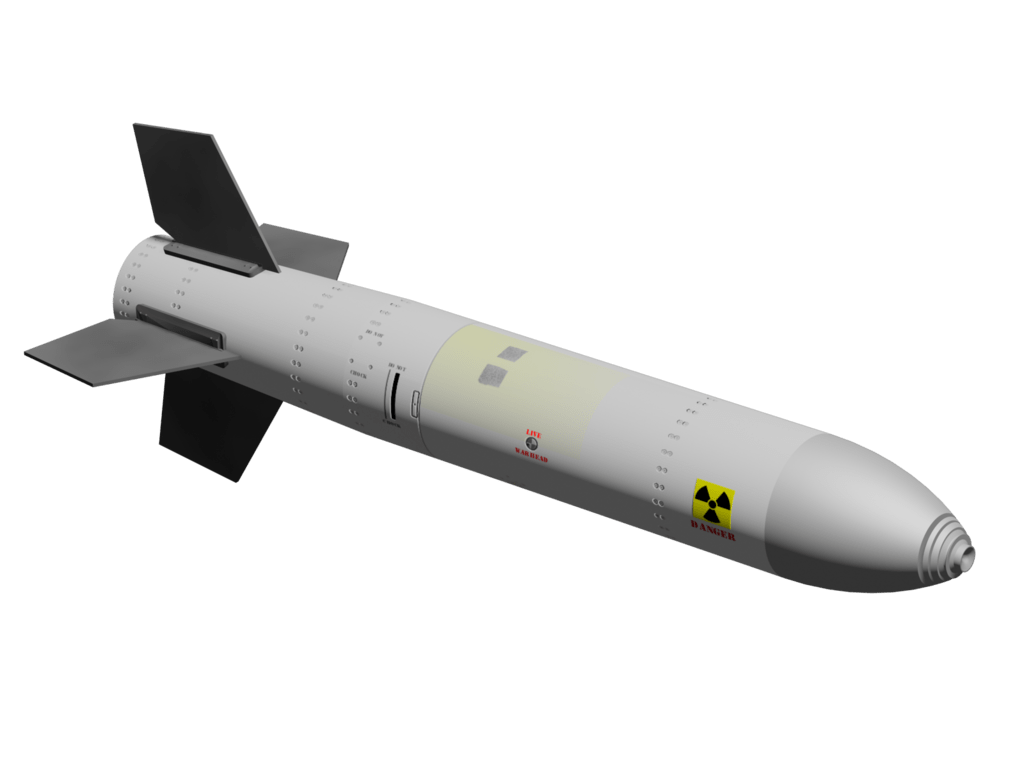
\includegraphics[width=0.9\textwidth]{missile.png}}
	    		\end{figure}
		\end{column}
	\end{columns}
	\begin{figure}
	\begin{columns}
		\begin{column}{0.33\textwidth}
		\end{column}
		\begin{column}{0.33\textwidth}
	   	 	\begin{figure}
	   		 \centering
	      		 \uncover<5->{
\includegraphics[width=0.5\textwidth]{cargo.png}}
	    		\end{figure}
		\end{column}
		\begin{column}{0.33\textwidth}
	    		\begin{figure}
	   		 \centering
	      		 \uncover<6->{
\includegraphics[width=0.6\textwidth]{helicopter_ban.png}}
	    		\end{figure}
		\end{column}
	\end{columns}
	\end{figure}
\end{frame}

\subsection{Cel projektu}
\begin{frame}%[allowframebreaks]
	\frametitle{Cel projektu}
	  \begin{itemize}
	  \item {
	    Kompleksowa symulacja fizyki.
	    \pause % Tu nastąpi pauza
	  }
	  \item {   
	    Wysoka konfigurowalność BSP, środowiska i symulacji.
	  }
	  % Można ustalić kiedy dany element ma się pojawić, używając <n->:
	  \item<3-> {
	    Bogate narzędzia dla analityków.
	  }
	  \item<4-> {
	    Licencja open-source.
	  }
 	 \end{itemize}
\end{frame}

\section{Wstep teoretyczny}
\begin{frame}%[allowframebreaks]
	\frametitle{Wstep teoretyczny}
	 \uncover<2->{\epigraph{There is nothing so practical as a good theory.}{Lewin Kurt}}
	 \uncover<3->{\epigraph{Nie ma osobnej ani teorii, ani praktyki inżynierskiej, jest tylko wspólna sztuka inżynierska.}{prof. Jan Oderfeld}}
\end{frame}


\subsection{Dynamika statku powietrznego}
\begin{frame}%[allowframebreaks]
	\frametitle{Dynamika lotu}
	\begin{columns}
		\begin{column}{0.55\textwidth}
	   	 	\begin{figure}
	   		 \centering
	      		 \uncover<2->{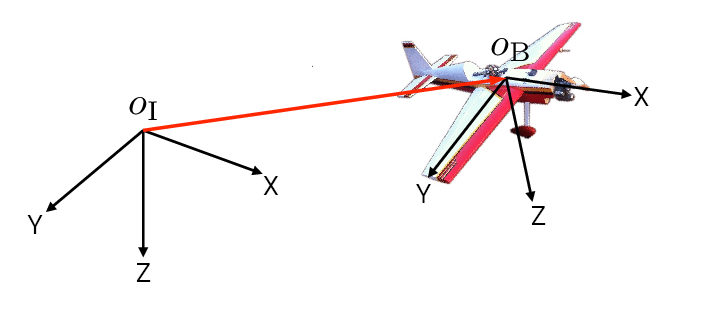
\includegraphics[width=1.05\textwidth]{frames.png}}
	    		\end{figure}
		\end{column}
		\begin{column}{0.45\textwidth}
	   	 	\begin{figure}
	   		 \centering
	      		 \uncover<3->{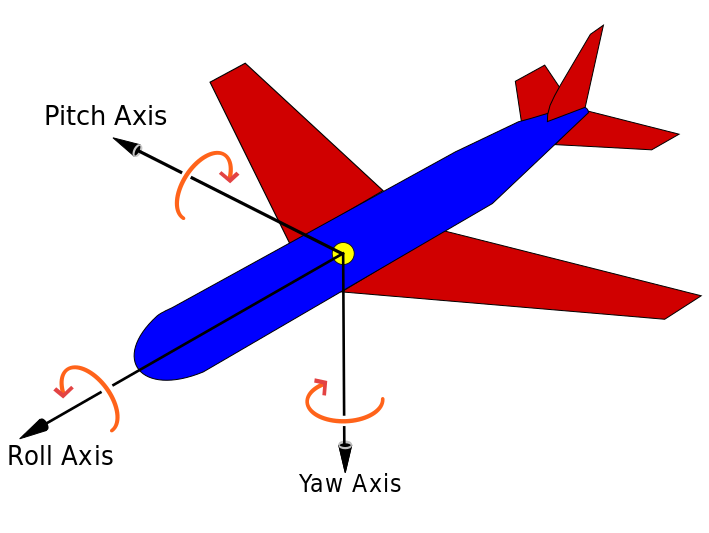
\includegraphics[width=1.05\textwidth]{RPY.png}}
	    		\end{figure}
		\end{column}
	\end{columns}
\end{frame}

\begin{frame}%[allowframebreaks]
	\frametitle{Równania stanu}
	\begin{columns}
		\begin{column}{0.3\textwidth}
	      		 	\uncover<1->{\[
				\begin{cases}
					\dot{\bm{x}} \left(t\right)  = \bm{Ax} \left(t\right)  + \bm{Bu} \left(t\right) \\
					\bm{y} \left(t\right) = \bm{Cx} \left(t\right) + \bm{Du} \left(t\right)
				\end{cases}
				\]}	
	      		 	\[
				\begin{cases}
					\dot{\bm{x}} \left(t\right)  = \bm{f} \left(t,\bm{x}\left(t\right),\bm{u}\left(t\right) \right) \\
					\bm{y} \left(t\right) = \bm{g} \left(t,\bm{x}\left(t\right),\bm{u}\left(t\right) \right)
				\end{cases}
				\]	
		\end{column}
		\begin{column}{0.7\textwidth}
	   	 	\begin{figure}
	   		 \centering
	      		 \uncover<2->{\includegraphics[width=0.9\textwidth]{state\_eq.png}}
	    		\end{figure}
		\end{column}
	\end{columns}
\end{frame}

\begin{frame}%[allowframebreaks]
	\frametitle{Równania różniczkowe}
	\begin{itemize}
	  \item{
	    Przed zastosowaniem algorytmu obniżyć rząd równania różniczkowego.
	    \pause
	  }
	  \item {   
	    Skorzystać z algorytmu jawnego lub niejawnego algorytmu całkowania RR
	    \pause
	  }
	  % Można ustalić kiedy dany element ma się pojawić, używając <n->:
	  \item {
	    Algorytmy jawne:
	    \pause
	    \begin{itemize}
		  \item{
		    Euler: $\bm{x}\left(t + \Delta t\right) = \bm{x}\left(t\right) + \Delta t \cdot \bm{\dot{x}} $
		    \pause
		  }
		  \item {   
		    Rugge-Kutty 4 rzędu
		  }
	     \end{itemize}
	     \pause
	  }
	  \item {   
	    Algorytmy niejawne
	  }
 	 \end{itemize}
\end{frame}

\begin{frame}%[allowframebreaks]
	\frametitle{Model matematyczny statku powietrznego I}
	\begin{columns}[T]
		\begin{column}{0.33\textwidth}
	   	 	\begin{figure}
	      		 \uncover<2->{
	      		 Położenie i orientacja:
	      		  \begin{center}
	      		 \[
	      		 \bm{y} = \begin{bmatrix}x\\y\\z\\ \varphi \\ \Theta \\ \Psi  \end{bmatrix}_{W} \text{lub} \begin{bmatrix}x\\y\\z\\ q_0 \\ q_x \\ q_y \\ q_z  \end{bmatrix}_{W}
	      		 \]
	      		  \end{center}}
	    		\end{figure}
		\end{column}
		\begin{column}{0.33\textwidth}
	   	 	\begin{figure}
	      		 \uncover<3->{
	      		 Prędkości:
	      		  \begin{center}
	      		 \[
	      		 \bm{x} = \begin{bmatrix}v_x\\v_y\\v_z\\ P \\ Q \\ R  \end{bmatrix}_{B}
	      		  \]
	      		   \end{center}}
	    		\end{figure}
		\end{column}
		\begin{column}{0.33\textwidth}
	    		\begin{figure}
	   		 \uncover<4->{
	   		 Stan układu:
	   		 \begin{center}
	      		 \[
	      		 \begin{bmatrix} \bm{y}\\ \bm{x} \\ \vdots \end{bmatrix}
	      		 \]
	      		  \end{center}}
	    		\end{figure}
		\end{column}
	\end{columns}	
\end{frame}

\begin{frame}%[allowframebreaks]
	\frametitle{Model matematyczny statku powietrznego II}
	\begin{columns}[T]
		\begin{column}{0.5\textwidth}
			 \begin{itemize}
			  \item<2-> {
			    Prędkość to pochodna położenia
			    \vspace{15pt}
			  }
			  \item<4-> {   
			    Zasada zmienności pędu i krętu, czyli uogólniona II zasada dynamiki Newtona
			    \[
		              \begin{bmatrix}\frac{d\bm{\vec{p}}}{dt}\\ \frac{d\bm{\vec{L}}}{dt} \end{bmatrix} = \begin{bmatrix}\bm{\vec{F}}\\ \bm{\vec{M}} \end{bmatrix} = \bm{f}
		              \]
			    }
			\end{itemize}
		\end{column}
		\begin{column}{0.5\textwidth}
	   	 	\begin{itemize}
			  \item<3->[] {
			   \[
			   	\bm{\dot{y}} = T(\bm{y}, \bm{x})
			   \]
			  }
			  \vspace{15pt}
			  
			  \item<5->[]{   
			    \[
			   	\bm{M} \bm{\dot{x}} +  \bm{\Omega} \left( \bm{x} \right) \bm{M} \bm{x} = \bm{f}
			   \]
			    }
			\end{itemize}
		\end{column}
	\end{columns}
\end{frame}

\begin{frame}%[allowframebreaks]
	\frametitle{Model matematyczny statku powietrznego III}
	Siły i momenty działające na samolot:
			 \begin{itemize}
			  \item<2-> {
			    Siła grawitacji  $\bm{f_G}$
			  }
			  \item<3-> {   
			    Ciąg silników i moment oporowy  $\bm{f_R}$
			   }
			    \item<3-> {   
			    Ciąg silników marszowych  $\bm{f_J}$
			   }
			    \item<4-> {   
			    Oddziaływanie aerodynamiczne $\bm{f_A}$
			   }
			    \item<5-> {   
			   Siły zewnętrzne $\bm{f_{OUT}}$
			   }
			\end{itemize}
\end{frame}

\begin{frame}%[allowframebreaks]
	\frametitle{Model matematyczny statku powietrznego IV}
	Ciąg silnika i moment oporowy:
	\begin{columns}
		\begin{column}{0.5\textwidth}
	   	 	\begin{figure}
	   		 \centering
	      		 \uncover<2->{
	      		 \[
	      		 	F = k_F \rho S R^2 \omega^2
			\]}
			 \uncover<3->{
	      		 \[
	      		 	M = k_M \rho S R^3 \omega^2
	      		\]} 
	    		\end{figure}
		\end{column}
		\begin{column}{0.5\textwidth}
	   	 	\begin{figure}
	   		 \centering
	      		 \uncover<4->{ 
	      		 \[
	      		 	T \frac{d\omega}{dt} + \omega = \omega_{ZADANA}
	      		 \]}
	    		\end{figure}
		\end{column}
	\end{columns}
\end{frame}

\begin{frame}%[allowframebreaks]
	\frametitle{Model matematyczny statku powietrznego V}
	Ciąg silnika marszowego:
	   	 	\begin{figure}
	   		 \centering
	      		 \uncover<2->{\includegraphics[width=0.5\textwidth]{jet\_thrust.png}}
	    		\end{figure}
\end{frame}

\begin{frame}%[allowframebreaks]
	\frametitle{Model matematyczny statku powietrznego V}
	Oddziaływanie aerodynamiczne:
	\begin{columns}
		\begin{column}{0.4\textwidth}
	   	 	\begin{figure}
	   		 \centering
	      		 \uncover<2->{
	      		 \[
	      		 	\bm{f_A} = \frac{1}{2}\rho V_{T}^2  \bm{S} \bm{C}\left(\alpha, \beta, \bm{x}, \bm{\delta}, ... \right)
			\]}

	    		\end{figure}
		\end{column}
		\begin{column}{0.6\textwidth}
	   	 	\begin{figure}
	   		 \centering
	      		 \uncover<4->{ 
	      		 \[
	      		 	 \bm{C} \approx \bm{C0} + \frac{d\bm{C}}{d\alpha}\alpha + \frac{d\bm{C}}{d\beta}\beta + \frac{d\bm{C}}{d\beta}\beta + \frac{d\bm{C}}{d\bm{x}}\bm{x} + \frac{d\bm{C}}{d\bm{\delta}}\bm{\delta}
	      		 \]}
	    		\end{figure}
		\end{column}
	\end{columns}
\end{frame}


\begin{frame}%[allowframebreaks]
	\frametitle{Kolizje I}
	\begin{columns}
		\begin{column}{0.45\textwidth}
	   	 	\begin{figure}
	   		 \centering
	      		 \uncover<1->{\includegraphics[width=0.8\textwidth]{collision\_plane.png}}
	    		\end{figure}
		\end{column}
		\begin{column}{0.55\textwidth}
	   	 	\begin{figure}
	   		 \centering
	      		 \uncover<2->{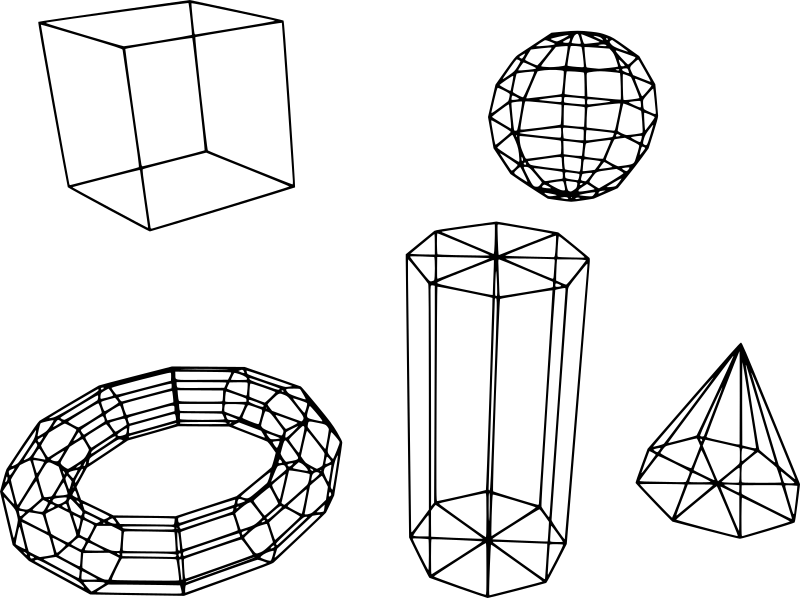
\includegraphics[width=0.9\textwidth]{meshes.png}}
	    		\end{figure}
		\end{column}
	\end{columns}
\end{frame}

\begin{frame}%[allowframebreaks]
	\frametitle{Kolizje II}
	\begin{columns}
		\begin{column}{0.5\textwidth}
	   	 	\begin{figure}
	   		 \centering
	      		 \uncover<2->{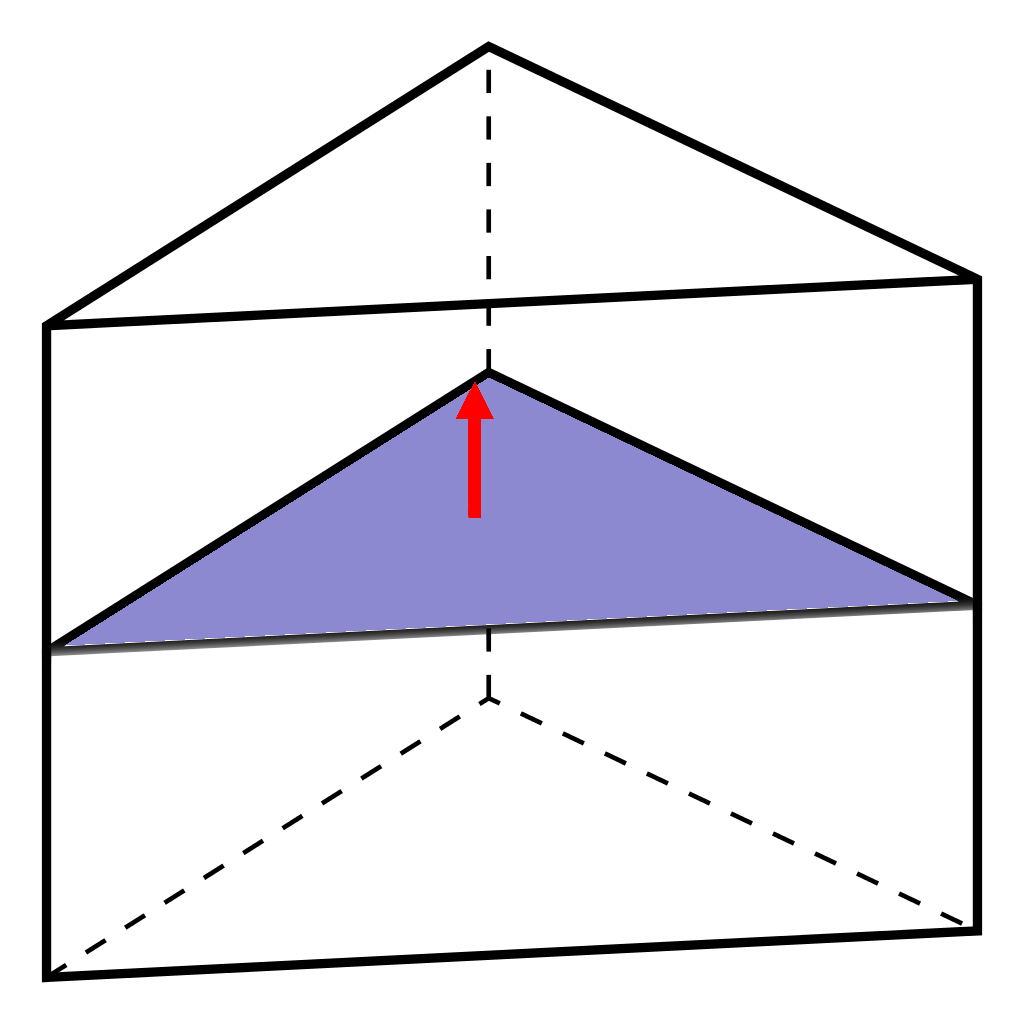
\includegraphics[width=0.85\textwidth]{prism.png}}
	    		\end{figure}
		\end{column}
		\begin{column}{0.5\textwidth}
	   	 	\begin{figure}
	   		 \centering
	      		 \uncover<3->{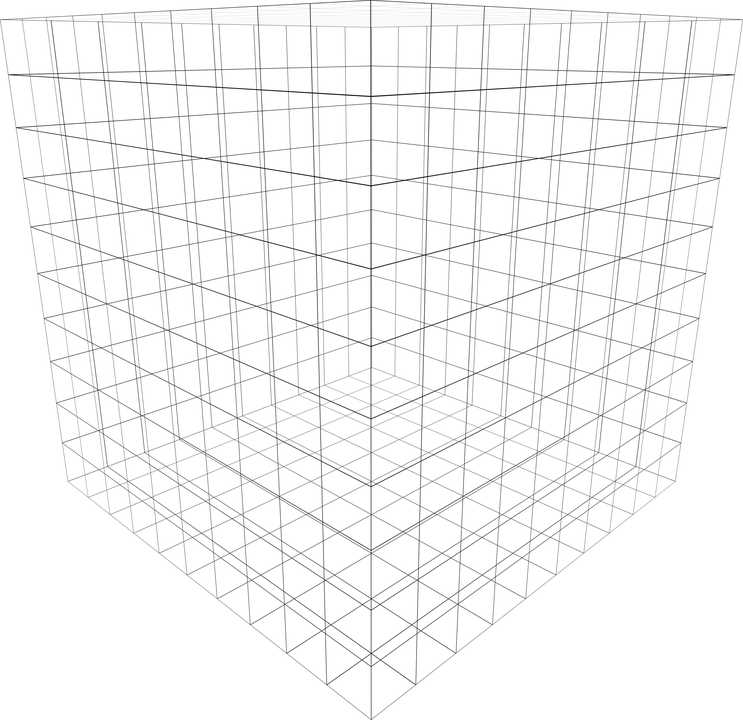
\includegraphics[width=0.9\textwidth]{grid.png}}
	    		\end{figure}
		\end{column}
	\end{columns}
\end{frame}


\begin{frame}%[allowframebreaks]
	\frametitle{Kolizje III}
	\begin{columns}
		\begin{column}{0.5\textwidth}
	   	 	\begin{figure}
	   		 \centering
	      		 \uncover<2->{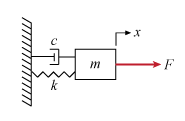
\includegraphics[width=0.9\textwidth]{oscillator.png}}
	    		\end{figure}
		\end{column}
		\begin{column}{0.5\textwidth}
	   	 	\begin{figure}
	   		 \centering
	      		 \uncover<3->{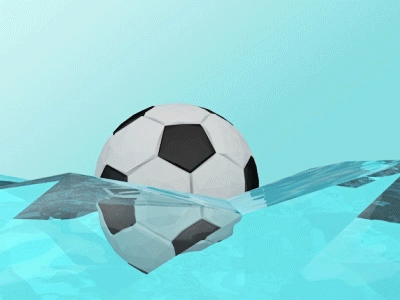
\includegraphics[width=0.9\textwidth]{ball.png}}
	    		\end{figure}
		\end{column}
	\end{columns}
\end{frame}


\begin{frame}%[allowframebreaks]
	\frametitle{Kolizje IV}
	\begin{columns}
		\begin{column}{0.4\textwidth}
			\begin{figure}
			\centering
		      		 \[
		      		 \bm{\vec{j}} = \int_{t_0}^{t_1} \bm{\vec{F}} dt
		      		 \]
		      		\pause
		      		\[
		      		j_r \left( \bm{M}, \bm{\vec{v}}, ...  , COR \right)
		      		\]
		      		\uncover<5->{
		      		\[
		      		j_f \left( \bm{M}, \bm{\vec{v}}, ...  , \mu_s, \mu_d \right)
		      		\]
		      		}	 
			\end{figure}
		\end{column}
		\begin{column}{0.6\textwidth}
	   	 	\begin{figure}
	   		 \centering
	      		 \uncover<4->{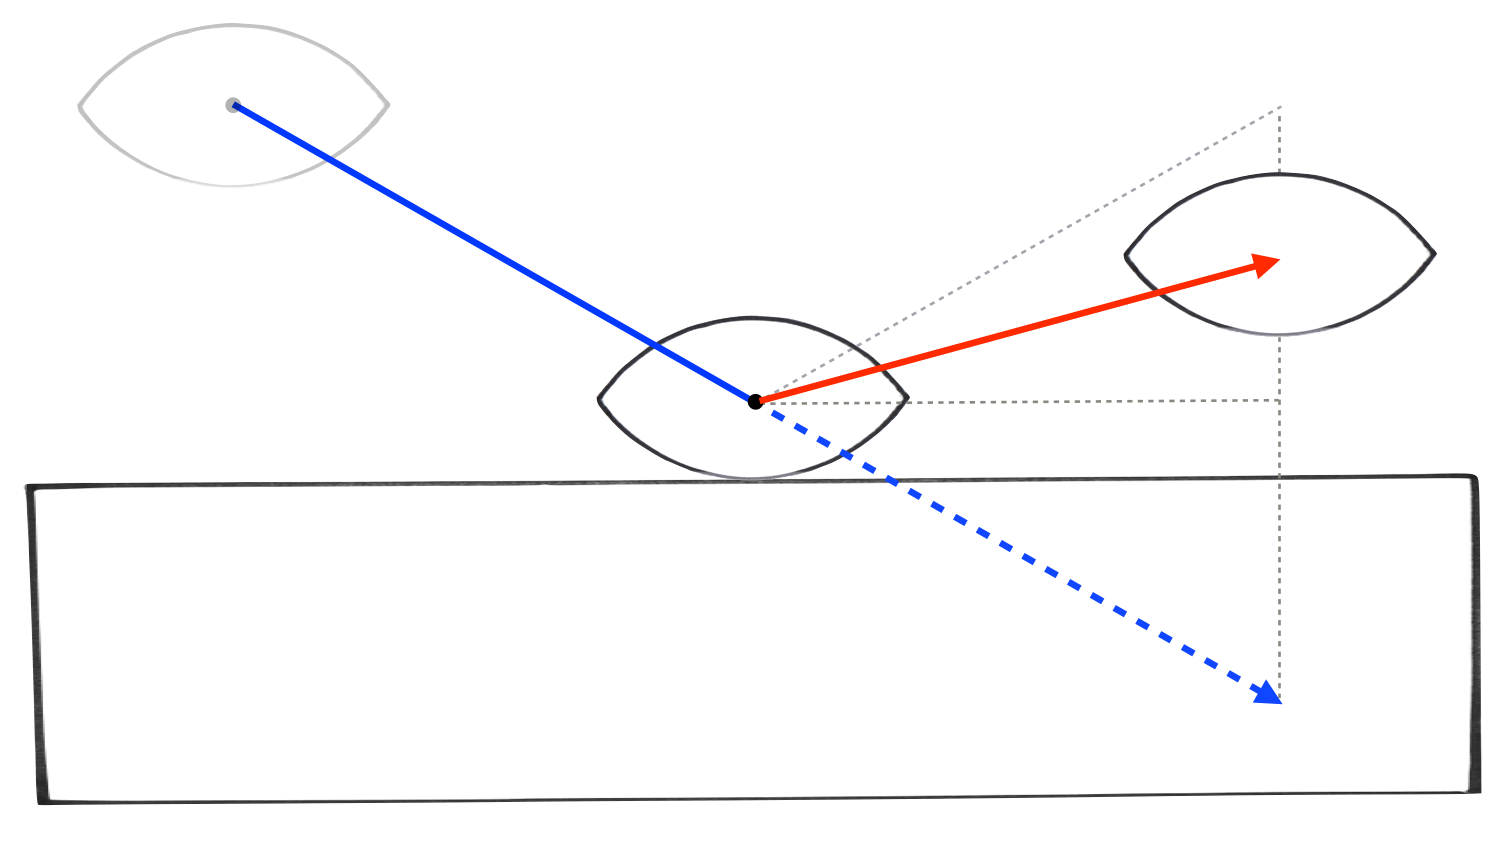
\includegraphics[width=0.9\textwidth]{cor.png}}
	    		\end{figure}
		\end{column}
	\end{columns}
\end{frame}


\begin{frame}%[allowframebreaks]
	\frametitle{Odrzut}
	\uncover<2->{Zasada zachowania pędu $\vec{\bm{p}}$ i zasada zachowania momentu pędu (krętu) $\vec{\bm{L}}$}.
	\uncover<3->{
	\[
		\begin{bmatrix}
		\vec{\bm{p}}_{przed}\\
		\vec{\bm{L}}_{przed}
		\end{bmatrix}
		=
		\begin{bmatrix}
		\vec{\bm{p}}_{po}\\
		\vec{\bm{L}}_{po}
		\end{bmatrix}
		+	
		\begin{bmatrix}
		\vec{\bm{p}}_{pocisku}\\
		\vec{\bm{L}}_{pocisku}
		\end{bmatrix}	
	\]}
	\uncover<4->{
	\[
		\bm{M}
		\begin{bmatrix}
		\vec{\bm{v}}_{przed}\\
		\vec{\bm{\omega}}_{przed}
		\end{bmatrix}
		=
		\bm{M}
		\begin{bmatrix}
		\vec{\bm{v}}_{po}\\
		\vec{\bm{\omega}}_{po}
		\end{bmatrix}
		+
		m_{pocisku}
		\begin{bmatrix}
		\vec{\bm{v}}_{pocisku}\\
		\vec{\bm{r}}_{pocisku} \times  \vec{\bm{v}}_{pocisku}
		\end{bmatrix}	
	\]}
	
\end{frame}

\subsection{Sterowanie statkiem powietrznym}

\begin{frame}
	\frametitle{Sterowanie statkiem powietrznym}
	\begin{figure}
	   		 \centering
	      		 \uncover<2->{\includegraphics[width=0.9\textwidth]{uk\_reg.jpg}}
	\end{figure}
\end{frame}
\begin{frame}
	\frametitle{Sterowanie statkiem powietrznym}
	\begin{figure}
	   		 \centering
	      		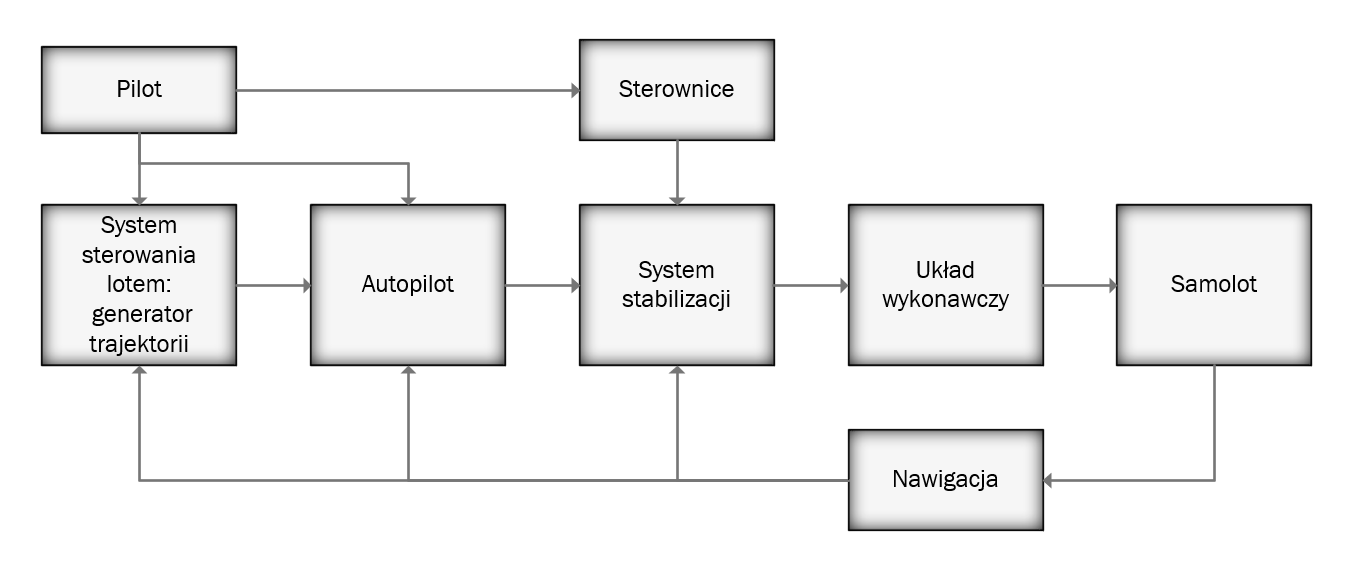
\includegraphics[width=\textwidth]{controller.png}
	\end{figure}
\end{frame}

\begin{frame}%[allowframebreaks]
	\frametitle{Regulator PID}
	\begin{columns}
		\begin{column}{0.5\textwidth}
	   	 	\begin{figure}
	   		 \centering
	      		 \uncover<2->{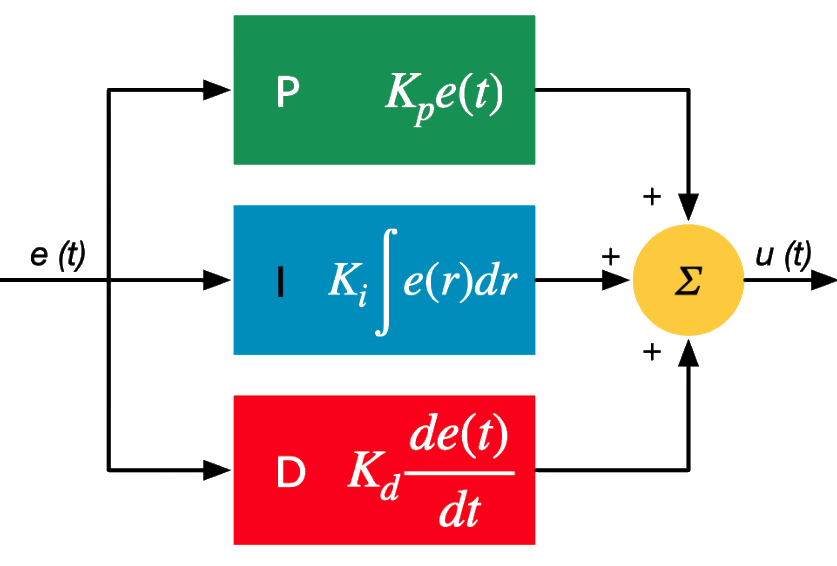
\includegraphics[width=\textwidth]{pid.png}}
	    		\end{figure}
		\end{column}
		\begin{column}{0.5\textwidth}
	   	 	\begin{figure}
	   		 \centering
	      		 \uncover<3->{\includegraphics[width=\textwidth]{pid\_graph.png}}
	    		\end{figure}
		\end{column}
	\end{columns}
	
	
\end{frame}

\begin{frame}
	\frametitle{Sterowanie statkiem powietrznym}
	\begin{figure}
	   		 \centering
	      		 \includegraphics[width=1.05\textwidth]{pid\_cascade.jpg}
	\end{figure}
\end{frame}

\begin{frame}%[allowframebreaks]
	\frametitle{Nawigacja}
	\begin{columns}[T]
		\begin{column}{0.5\textwidth}
	   	 	 Czujniki:
	   	 	 \begin{itemize}
			  \item{
			    Żyroskop
			    \pause
			  }
			  \item {   
			    Akcelerometer
			    \pause
			  }
			  \item {   
			    Barometer
			    \pause
			  }
			  \item {   
			    Czujnik prędkości powietrza
			    \pause
			  }
			  \item {   
			    Nawigacja satelitarna
			    \pause
			  }
			  \item {   
			    Radar, sonar, lidar
			  }
	     \end{itemize}
	     \pause
	   	 	
		\end{column}
		\begin{column}{0.5\textwidth}
			Filtr Kalmana:
	   	 	\begin{figure}
	   		 \centering
	      		 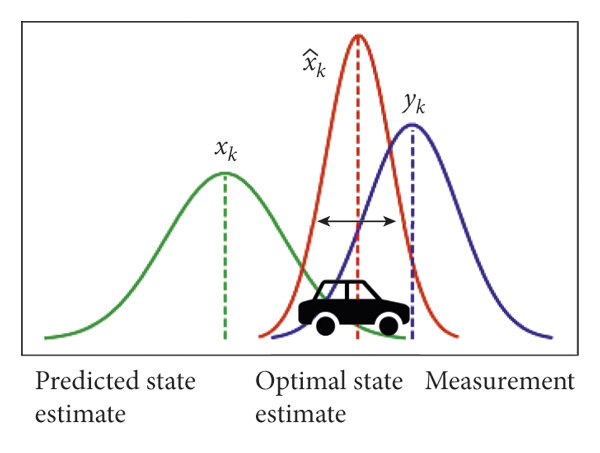
\includegraphics[width=0.8\textwidth]{kalman.png}
	    		\end{figure}
		\end{column}
	\end{columns}
\end{frame}

\subsection{Grafika komputerowa}

% Wprowadzając grafikę komputerową, nie można nie wpsomnieć o GPU, a więc procesorach graficznych. Jak nazwa wskazuje zostały one początkowo wprowadzone na rynek by programy były sobie w stanie radzić z wykonywaniem rzędy wielkości operacji więcej niż to co jest możliwe na zwykłym procesorze. 
\begin{frame}
\frametitle{GPU}
	\begin{figure}
		\centering
		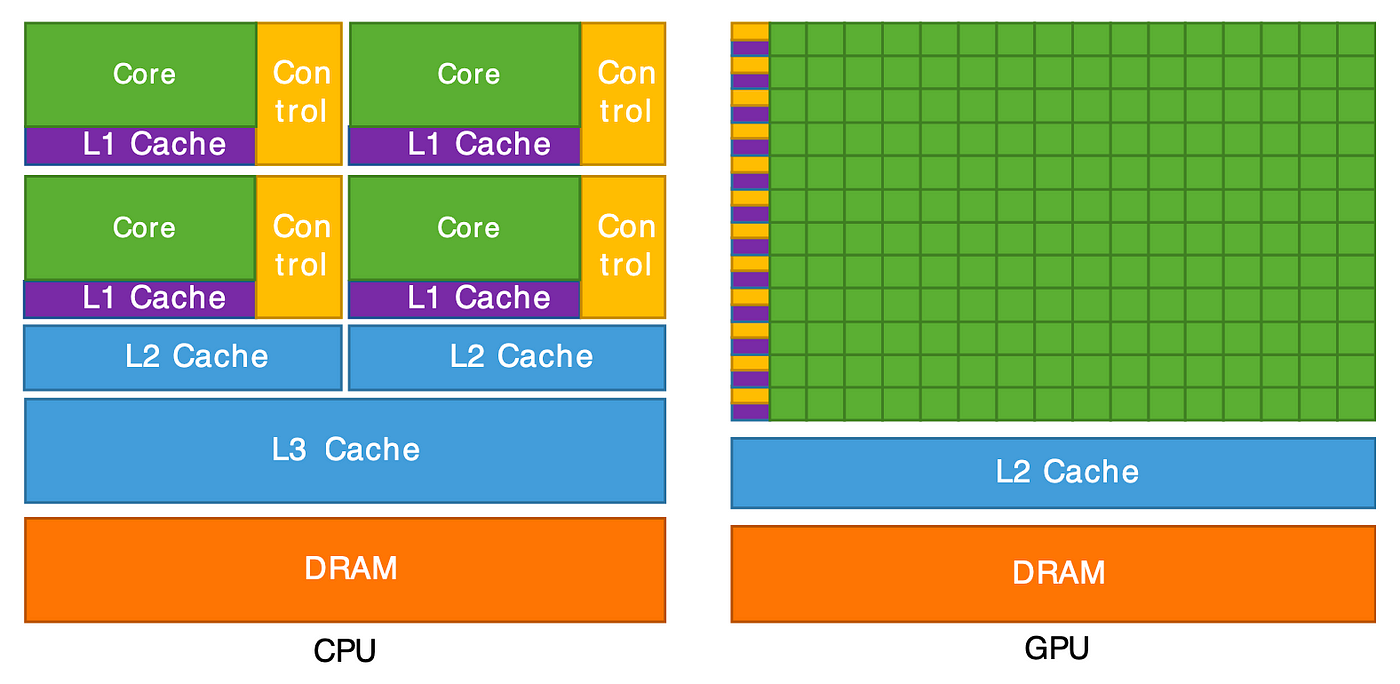
\includegraphics[width=0.8\textwidth]{gpu.png}
	\end{figure}
\end{frame}

% OpenGL czyli Open Graphics Libraru, jest uniwersalnym interfejsem do renderowania grafiki werktorowej 2D i 3D wykorzystującym GPU. Za specyfikację OpenGL odpowiada Khronos Group, a za implementację funkcji najczęściej producenci kart graficznych. W praktyce jest to olbrzymia maszyna stanu, która definiuje sposób działania OpenGL. Aby stan zmieniać operujemy na obiektach, które przypisujemy do kontekstu. [Opisać obrazek]
\begin{frame}
\frametitle{OpenGL}
	\begin{figure}
		\centering
		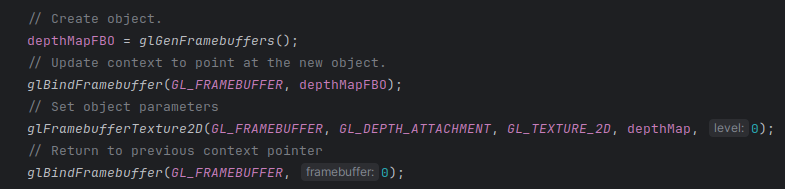
\includegraphics[width=0.9\textwidth]{OpenGL_example.png}
	\end{figure}
\end{frame}

% Przetwarzanie wierzchołków
% Każdy obiekt w scenie składa się z wierzchołków. Atrybuty tych wierzchołków (np. położenie) poddawane są przekształceniom. []Narysować dwa obiekty takie same jak przechodzą na płaszczyznę ekran]. (Mamy na to wpływ w Vertex Shader)
% Łączenie w prymitywy
% [Pokazać trójkąty]
% Przycinanie
% Rasteryzacja
% Tworzone są fragmenty, czyli próbki powierzchni prytmitywu, któremu odpowiada piksel bufora klatki. Może być wiele fragmentów na jeden piksel. W tym momencie dane wierzchołka są interpolowane, w przypadku trójkąta, z trzech wierzchołków. 
% Przetwarzanie fragmentów.
% Dodawanie tekstury, oświetlenie. (Mamy na to wpływ w Fragment Shader)
% Przetwarzanie piksli
% Tutaj zachodzi test głębokości, alpha blending czyli przezroczystość i antialiasing.

% Teraz opiszemy to na co mamy wpływ, a więc dane, przetwarzanie wierzchołków i fragmentów.
\begin{frame}
\frametitle{Potok renderowania}
		\begin{figure}
			\centering
			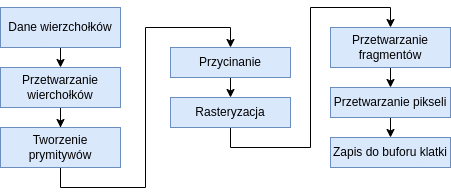
\includegraphics[width=0.7\textwidth]{graphics_pipeline.png}
		\end{figure}
\end{frame}

% Porozumiewanie się z procesrowem graficznym wymaga jednak własnego języka. W przypadku OpenGLa, jest nim GLSL ,,OpenGl Shading Language''. Został on zaprojektowany na bazie C, nakładając duży poziom abstrakcji na operacje wykonywane na GPU. Pisząc shadery właściwie się nie myśli o równoległości. [Opis języka]
\begin{frame}[allowframebreaks]
	\frametitle{Shadery}
	\begin{figure}
		\centering
		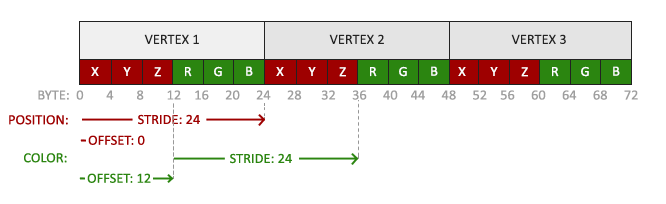
\includegraphics[width=0.8\textwidth]{vertex_attributes.png}
	\end{figure}
	\framebreak
	
	\begin{figure}
		\centering
		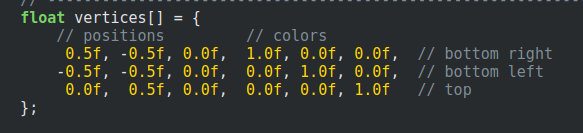
\includegraphics[width=0.8\textwidth]{vertex.png}
	\end{figure}
	\framebreak
	
	\begin{columns}
		\begin{column}{0.5\textwidth}
			\begin{figure}
				\centering
				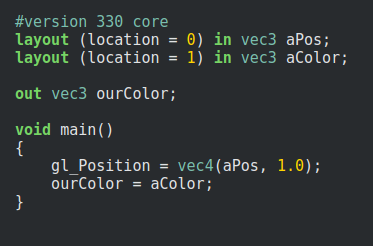
\includegraphics[width=0.9\textwidth]{vertex_shader.png}
			\end{figure}
		\end{column}	
		
		\begin{column}{0.5\textwidth}
			\begin{figure}
				\centering
				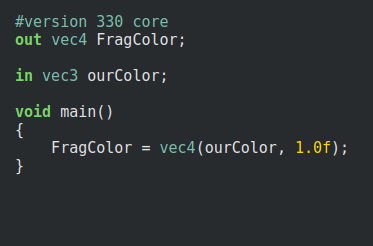
\includegraphics[width=0.9\textwidth]{fragment_shader.png}
			\end{figure}
		\end{column}
	\end{columns}
	\framebreak
	
	\begin{figure}
	\centering
	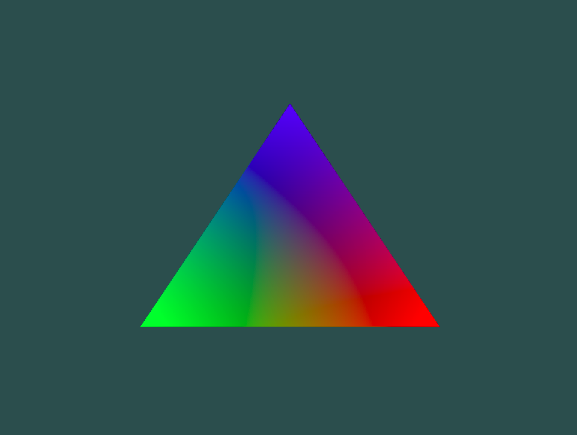
\includegraphics[width=0.6\textwidth]{shader_result.png}
	\end{figure}
\end{frame}

% Cieniowanie w grafice komputerowej możemy wykonywać na różne sposoby. 
% Od lewej mamy:
% Kolorowanie płaskie - tutaj oświetlenie ustalamy na poziomie prymitywu.
% KOlorwanie Gourauda - Tutaj ustalamy oświetlenie na poziomie wierzchołków i je interpolujemy.
% Kolorowanie Phonga - Tutaj interpolujemy wektory normalne. Obliczenie koloru następuje dla każdego fragmentu.
\begin{frame}[allowframebreaks]
	\frametitle{Cieniowanie i model oświetlenia}	
	\begin{figure}
		\centering
		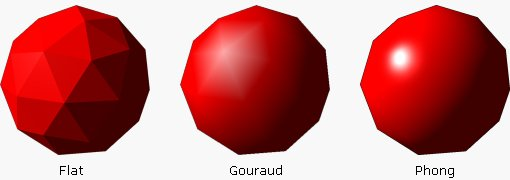
\includegraphics[width=0.7\textwidth]{shading.jpg}
	\end{figure}
	\framebreak
	\begin{figure}
		\centering
		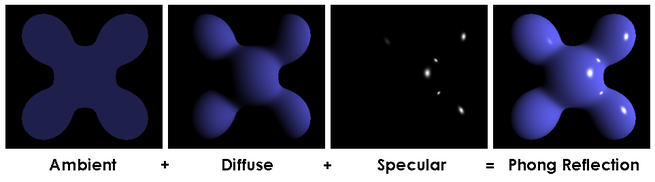
\includegraphics[width=0.9\textwidth]{phong.png}
	\end{figure}
\end{frame}

% \begin{frame}[allowframebreaks]
% 	\frametitle{Renderowanie interfejsu}
%	
% \end{frame}

% Istotnym elementem symulacji jest również interakcja z użytkownikiem.
% W naszym przypadku większość komunikacji odbywa się za pomocą kontrolera.
% System interpretuje każdy kontroler jako tablicę stanów przycisków, osi oraz hatów (d-padów).
% Niestety za jakie przyciski odpowiadają jakie indeksy, nie wiadomo. Zależy to od producenta kontrolera i trudno jest o jakiś standard w przypadku tylu różnych możliwości układu przycisków. 
% Są bazy danych, które pozwalają na mapowanie znanych modeli kontrolerów do konkretnych akcji, ale my chcemy umożliwić wykrozystanie najróżniejszych sprzętów. Od zwykłego pada do xboxa, po dedykowany kontroler do BSP.
% Rozwiązanie tego problemu nie jest takie trudne, chociaż pracochłonne. Wystarczy stworzyć interaktywną konfigurację, z której pomocą użytkownik sam będzie w stanie ustawić dedykowane bindingi.
\begin{frame}[allowframebreaks]
	\frametitle{Obsługa kontrolera}
	
	\begin{columns}
		\begin{column}{0.33\textwidth}
			\begin{figure}
				\centering
				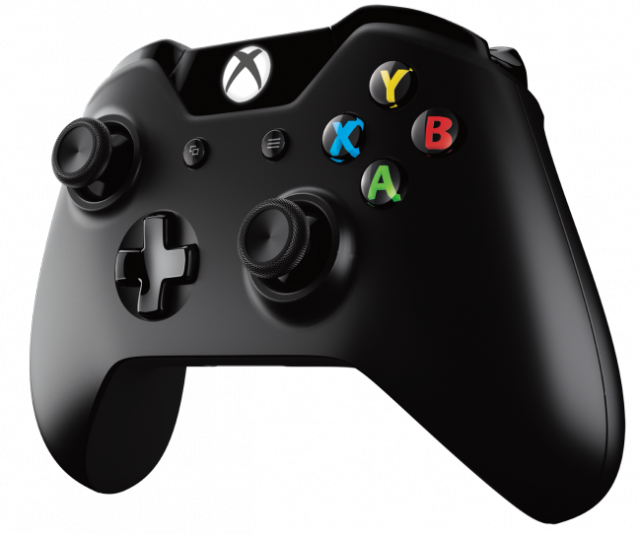
\includegraphics[width=0.7\textwidth]{xobx.png}
			\end{figure}
		\end{column}
		\begin{column}{0.33\textwidth}
			\begin{figure}
				\centering
				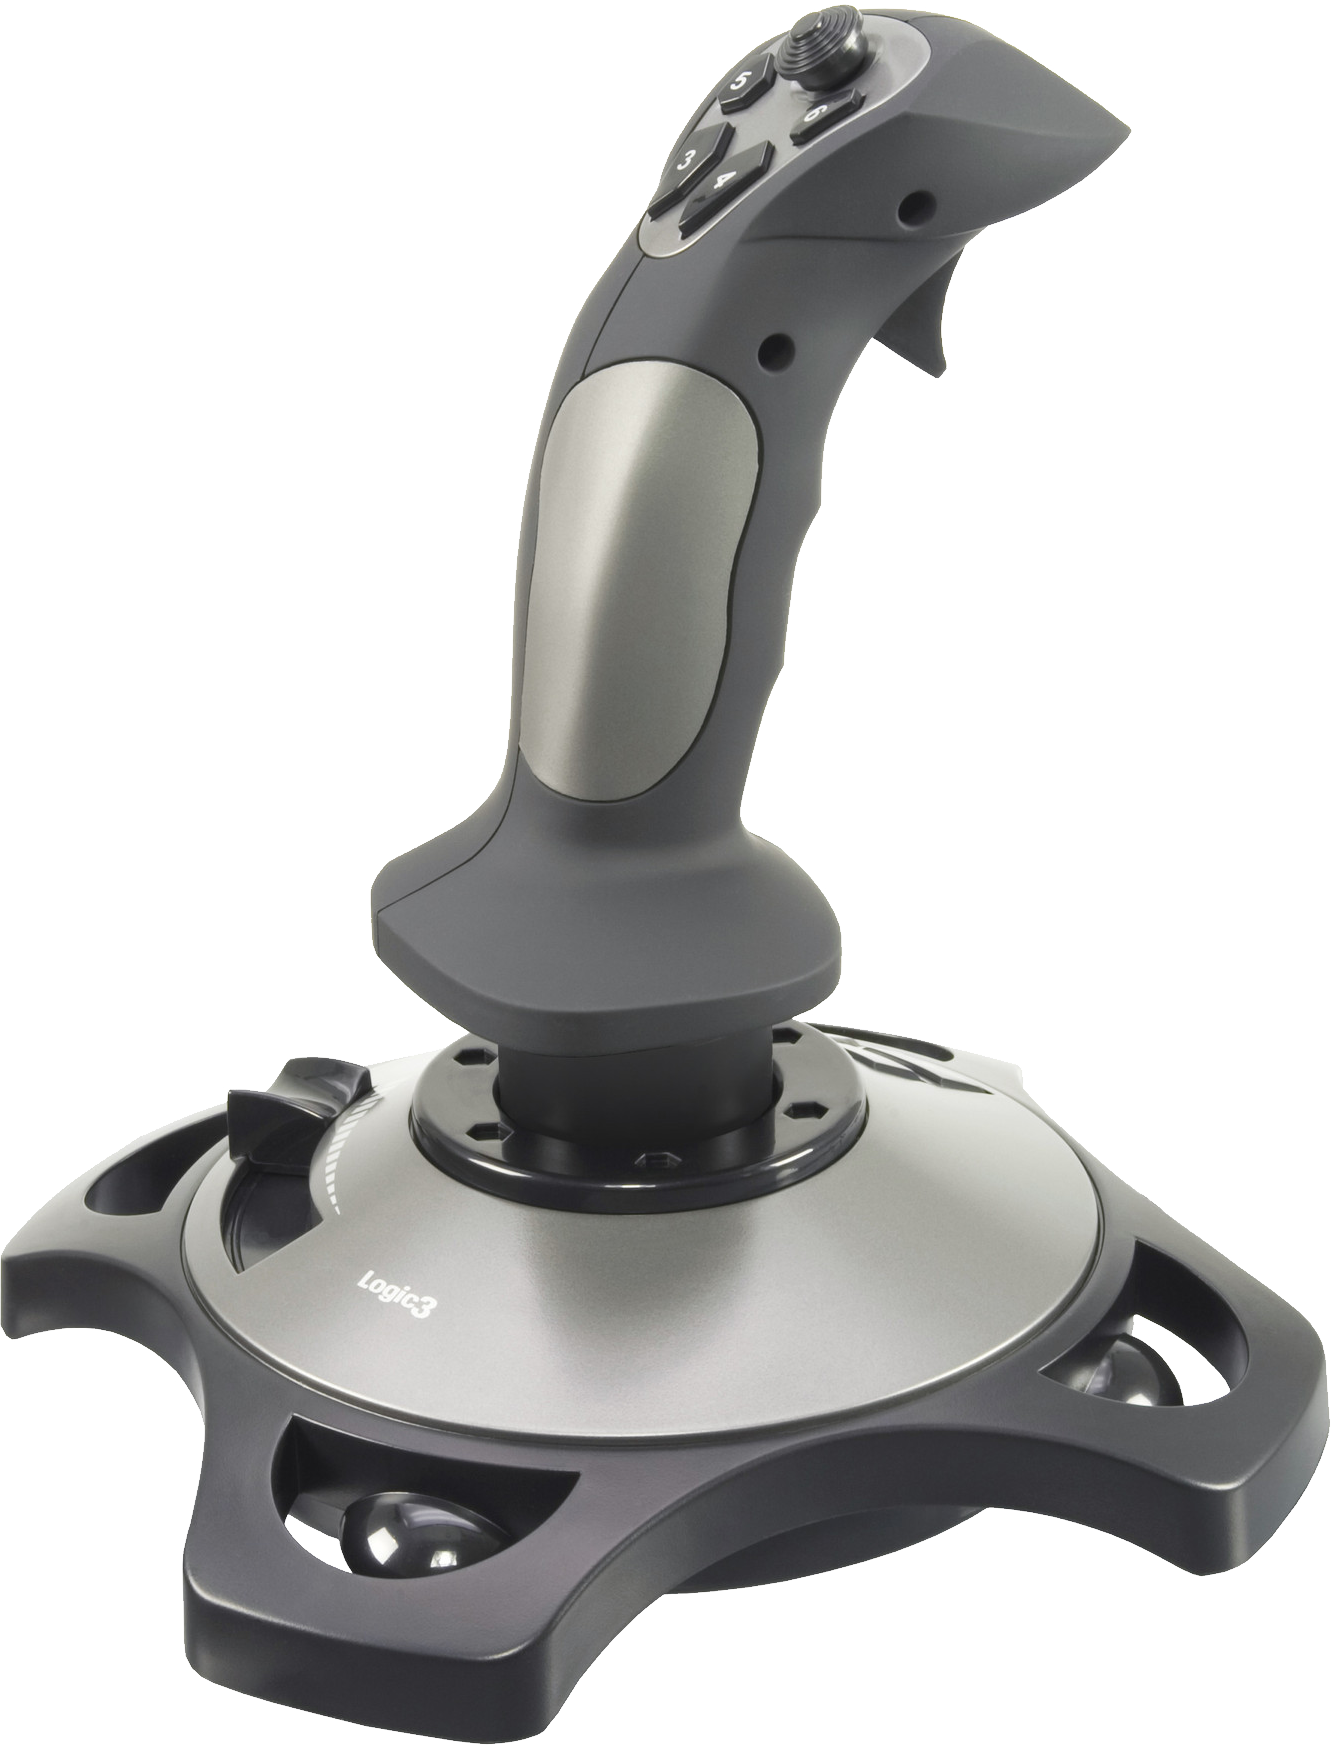
\includegraphics[width=0.7\textwidth]{joysticke.png}
			\end{figure}
		\end{column}
		\begin{column}{0.33\textwidth}
			\begin{figure}
				\centering
				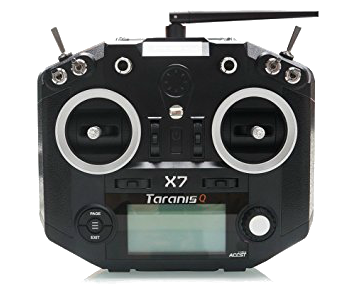
\includegraphics[width=0.7\textwidth]{taranis.png}
			\end{figure}
		\end{column}
	\end{columns}
	
	\begin{figure}
		\centering
		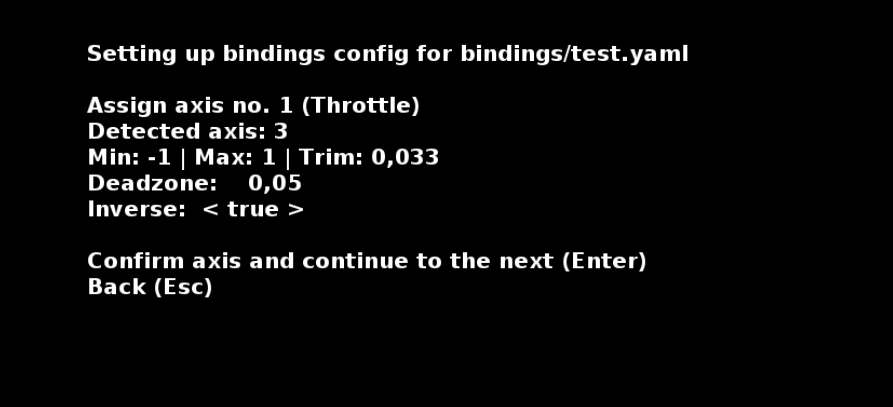
\includegraphics[width=0.8\textwidth]{bindings.png}
	\end{figure}
\end{frame}

\begin{frame}[allowframebreaks]
	\frametitle{Krzywa łańcuchowa}
	\begin{figure}
		\centering
		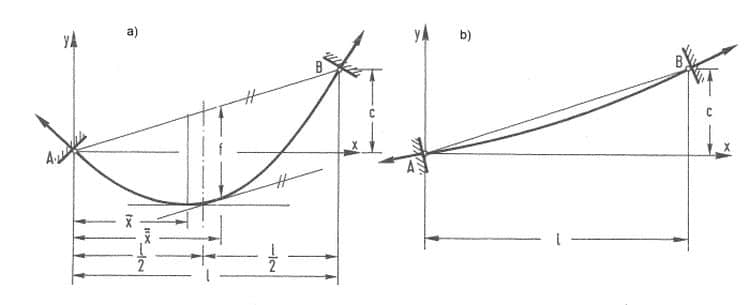
\includegraphics[width=0.7\textwidth]{catenary.jpg}
	\end{figure}
	$$\text{cat}(x) = a\cdot \cosh \left(\frac{x}{a}\right).$$
	
	\framebreak
	
	Wyznaczenie współczynnika krzywej łańcuchowej $a_c$ między punktami $A = (x_1,y_1)$, $B = (x_2,y_2)$ i danego $l < \lVert B - A \rVert$, to rozwiązanie równania:
	\begin{equation}
		\label{cat}
		\frac{1}{h} \sqrt{l^2-v^2} = \frac{2a_c}{h} \sinh\left( \frac{h}{2a_c} \right),
	\end{equation}
	gdzie:
	$$
	v = x_2 - x_1,
	$$
	$$
	h = y_2 - y_1.
	$$
	
	\framebreak
	Dla $l \geq \lVert B - A \rVert$ stosowany jest wzór na współczynnik kierunkowy prostej
	\begin{equation}
		\label{line}
		a_l = \frac{y_2 - y_1}{x_2 - x_1}.
	\end{equation}
	
	
	\framebreak
	Ostatecznie, dla danej długości liny $l \in \mathbb{R}$ oraz punktów $A$, $B  \in \mathbb{R}^2$ funkcja liny $f_l$ ma postać:
	$$f_l(x) = 
	\begin{cases}
		a_c \cdot \cosh\left( \frac{x}{a_c} \right), & l < \lVert B - A \rVert \\
		a_l \cdot x, & l \geq \lVert B - A \rVert 
	\end{cases},$$
	gdzie $a_c$ oraz $a_l$ są wyznaczone z równań \ref{cat} oraz \ref{line} dla punktów $A$ i $B$.
	
	\framebreak
	
	\begin{figure}
		\centering
		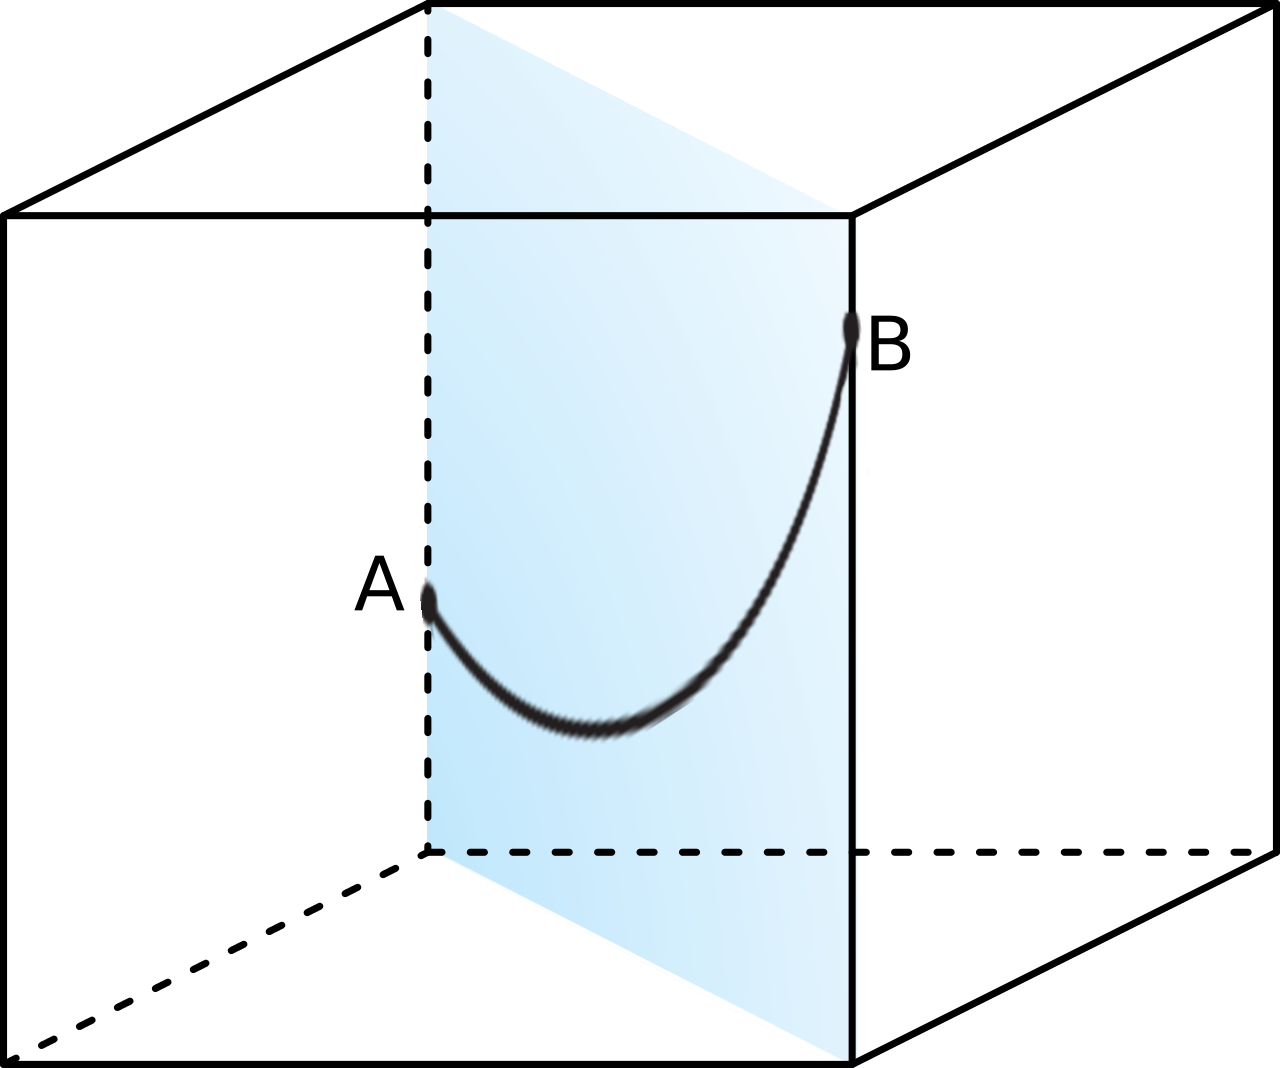
\includegraphics[width=0.4\textwidth]{cube.png}
	\end{figure}
	\framebreak
	
	
	\begin{columns}
		\begin{column}{0.5\textwidth}
			\begin{figure}
				\centering
				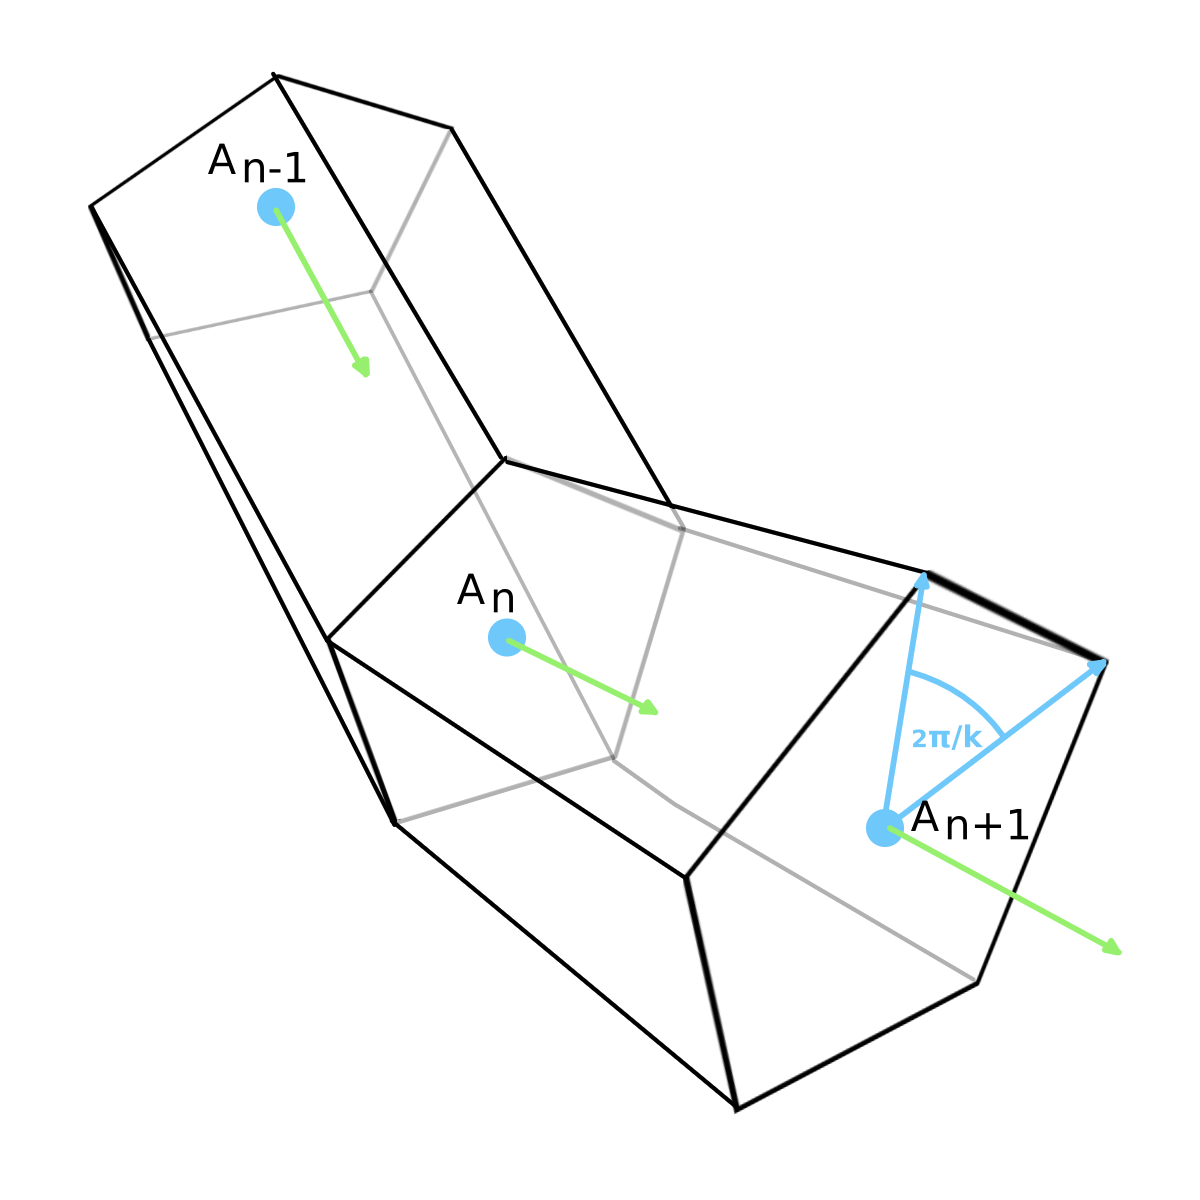
\includegraphics[width=1\textwidth]{rope_model.png}
			\end{figure}
		\end{column}	
		
		\begin{column}{0.5\textwidth}
				\begin{equation*}
				\frac{d}{dx} \text{cat}(x) = \frac{d}{dx} \left( a\cdot \cosh\left( \frac{x}{a} \right) \right) = \sinh\left( \frac{x}{a} \right)
			\end{equation*}
			\begin{equation*}
				\vec{t} =
				\begin{bmatrix}
					1 \cdot \frac{|\vec{l_x}|}{\vec{|l_{xy}}|}, &
					1 \cdot \frac{|\vec{l_y}|}{\vec{|l_{xy}}|}, &
					-\sinh(\frac{(x+x_{offset})}{a})
				\end{bmatrix}^T
			\end{equation*}
			\begin{equation*}
			\vec{n_0} =
			\begin{bmatrix}
				\sinh(\frac{(x+x_{offset})}{a}) \cdot \frac{|\vec{l_x}|}{\vec{|l_{xy}}|}, &
				\sinh(\frac{(x+x_{offset})}{a}) \cdot \frac{|\vec{l_y}|}{\vec{|l_{xy}}|}, &
				1
			\end{bmatrix}^T
			\end{equation*}
			\begin{equation*}
				M_R = 
				\begin{bmatrix}
					0 & -\vec{t_z} & \vec{t_y} \\
					\vec{t_z} & 0 & -\vec{t_x} \\
					\vec{t_y} & \vec{t_x} & 0 \\
				\end{bmatrix}
			\end{equation*}
			\begin{equation*}
				\vec{n_i} = 1 \cdot M_R^i
			\end{equation*}
		\end{column}
	\end{columns}
	\framebreak
	
\end{frame}

\section{Demo}

\begin{frame}
	  \begin{center}
	\Huge Demo
	\end{center}
\end{frame}


\begin{frame}
	\frametitle{Testy $\alpha$} %JOKE
	\begin{figure}
		\centering
		
\includegraphics[width=0.7\textwidth]{dog.jpg}
	\end{figure}
\end{frame}


\begin{frame}
	\frametitle{Dyskusja}
	\begin{figure}
		\centering
		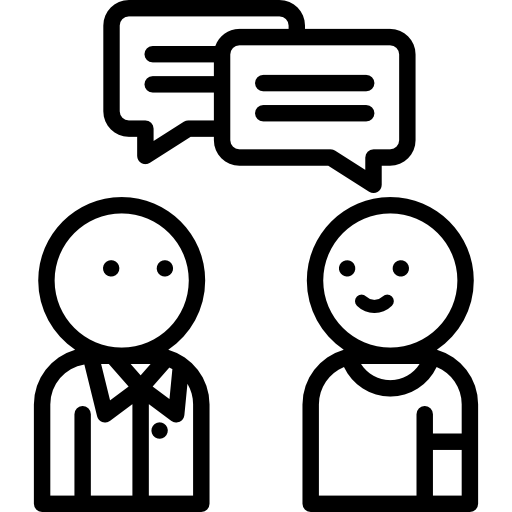
\includegraphics[width=0.7\textwidth]{questions.png}
	\end{figure}
\end{frame}

\begin{frame}{Literatura}
\begin{thebibliography}{10}
\beamertemplatebookbibitems
\bibitem{en15197136}[Energies, 2022] Quadrotor Model for Energy Consumption Analysis
   \newblock  Jacewicz, Mariusz and Żugaj, Marcin and Głębocki, Robert and Bibik, Przemysław
   
 \bibitem{cor} Collision Response and Coulomb Friction
 \newblock \url{https://gafferongames.com/post/collision_response_and_coulomb_friction/}
 
  \bibitem{openGL} Learn OpenGL
 \newblock \url{ https://learnopengl.com/}
 
  \bibitem{krzywa} Statyka cięgna
 \newblock \url{ https://chodor-projekt.net/encyclopedia/statyka-ciegna/}

\end{thebibliography}
\end{frame}

\begin{frame}
	  \begin{center}
	\Huge Dziękuje za uwagę!
	\end{center}
\end{frame}

\end{document}